% =====================================================================
% MDPI Aerospace paper
% "Pseudopilot Automation via LLM-Based Multi-Agent Systems
%  for ATC Training in X-Plane 12"
%
% Authors: Santiago Souto Ortega, Isaac González López
% =====================================================================

\documentclass[computers,article,submit,moreauthors,pdftex]{Definitions/mdpi}

% --- Metadata ---
\Title{Pseudopilot Automation via LLM-Based Multi-Agent Systems for ATC Training in X-Plane~12}
\Author{Santiago Souto Ortega$^{1,\dagger,\ddag}$\orcidA{}, Isaac Gonz\'{a}lez L\'{o}pez$^{2,\ddag}$\orcidB{}}
\AuthorNames{Santiago Souto Ortega, Isaac Gonz\'{a}lez L\'{o}pez}

\firstpage{1}
\makeatletter
\setcounter{page}{\@firstpage}
\makeatother

\address{%
    $^{1}$ \quad Affiliation 1; soutoortegasantiago@gmail.com \\
    $^{2}$ \quad Affiliation 2; isaac.gonzalez@example.com}

\corres{Correspondence: soutoortegasantiago@gmail.com}

% --- Abstract ---
\abstract{%
The training of air traffic controllers requires practice in simulators that
reproduce situations as closely as possible to those encountered in a real
control tower. In these exercises, the trainee issues radio instructions to the
aircraft present at the airport and must receive coherent and realistic
responses, just as would occur in real operations.

Currently, for this type of training to be possible, it is necessary to rely on
a team of people known as pseudopilots, whose task is to simulate the crews of
each aircraft. These operators respond to the controller's communications and
manage the movement of aircraft within the simulated environment. However, this
training model is costly, depends on the availability of qualified personnel,
and limits the number of sessions that can be carried out.

This work presents AIrport, a system that replaces pseudopilots with agents
capable of behaving like real pilots within a simulated airport. In the system,
the aircraft are represented by agents that interpret the received instructions,
respond over the radio using natural language, and manage aircraft movements
following real operational procedures.

The controller interacts with the system through voice and can observe the
result of their instructions in a three-dimensional representation of the
airport. In this way, a single person can carry out realistic exercises with
multiple aircraft simultaneously, without the need to mobilise a support team.
This reduces training costs and enables practice with greater frequency,
flexibility, and scalability.
}

\keyword{air traffic control; artificial intelligence; ATC training; aviation;
simulation; virtual assistants}

% =====================================================================
\begin{document}

% =====================================================================
\section{Introduction}
\label{sec:introduction}

Air traffic control (ATC) training has traditionally relied on human
pseudopilots — trained operators who simulate aircraft crews during simulation
exercises, responding to controller instructions and managing aircraft positions
within the simulated environment. The availability of qualified pseudopilots is
a bottleneck: training centres must maintain a roster of operators, coordinate
their schedules, and bear the recurring personnel cost. A student controller can
therefore only practise when both a simulator and a pseudopilot team are
available, limiting session frequency and total volume.

Recent advances in large language models (LLMs) and automatic speech recognition
(ASR) have opened the possibility of automating the pseudopilot role entirely:
an LLM-based agent can generate ICAO-compliant readbacks, and a speech-to-text
pipeline can replace the instructor who would otherwise type the controller's
words. Combined with a flight simulator capable of rendering aircraft motion,
this creates a self-contained training loop where a single controller trainee
speaks to a system that hears, understands, and responds with the correct
phraseology and the corresponding visual feedback.

This paper presents AIrport, an open-source platform that realises this vision.
The system integrates five components: (1)~a Whisper-based ASR pipeline with ATC
vocabulary correction; (2)~three LLM-based agents — one per controller position
(Delivery, Ground, Tower) — that generate ICAO readbacks and clearance data;
(3)~an orchestrator that tracks each aircraft's state machine across
DEL~$\rightarrow$~GND~$\rightarrow$~TWR transitions; (4)~a web-based controller
human-machine interface (HMI) with push-to-talk voice input, flight strips, and
ground radar; and (5)~an X-Plane~12 plugin that renders aircraft motion in a 3D
airport environment.

The contributions of this work are:
\begin{itemize}
    \item A complete, voice-driven ATC training loop that replaces human
          pseudopilots with LLM agents and replaces typed input with ASR.
    \item A quantitative benchmark of the ASR pipeline across three Whisper
          model sizes, three hardware configurations, and three context modes,
          establishing accuracy and latency bounds for live ATC use.
    \item A session-aware ASR correction pipeline that lifts entity-level
          accuracy (callsigns and SIDs) by 15--20~pp through decoder prompting
          and a deterministic-plus-LLM hybrid post-processor.
    \item An open-source release of the full system, including the
          pilot-readback-corpus dataset for ASR evaluation in ATC~\cite{SoutoReadbackCorpus2024}.
\end{itemize}

The remainder of the paper is organised as follows. Section~\ref{sec:related}
reviews related work on pseudopilot automation, ASR for ATC, and LLM-based
dialogue agents. Section~\ref{sec:materials} describes the materials and methods,
including the system architecture, the ATC agents, the X-Plane integration, and
the evaluation corpus. Section~\ref{sec:results} presents the experimental
results for both the ASR pipeline and the agent readback quality.
Section~\ref{sec:discussion} discusses the implications, limitations, and
practical deployment considerations. Section~\ref{sec:conclusions} concludes the
paper.

% =====================================================================
\section{Related Work}
\label{sec:related}

\subsection{Pseudopilot Automation}

[Placeholder — review of existing pseudopilot systems, speech-recognition-based
ATC simulators, and the gap this work fills.]

\subsection{ASR for Air Traffic Control}

[Placeholder — review of Whisper fine-tuning for ATC, ATCO2 corpus,
WER benchmarks in ATC domain, the challenge of domain-specific vocabulary.]

\subsection{LLM-Based Agents for Structured Dialogue}

[Placeholder — review of LLM agents, Google ADK, Gemini, structured output
generation, and prior work on aviation dialogue systems.]

% =====================================================================
\section{Materials and Methods}
\label{sec:materials}

\subsection{System Architecture}

[Placeholder — architecture diagram, service descriptions, data flow.]

% =====================================================================
% Section 3.1 — Automatic Speech Recognition
% MDPI Aerospace paper: "Pseudopilot Automation via LLM-Based
% Multi-Agent Systems for ATC Training in X-Plane 12"
% Authors: Santiago Souto Ortega, Isaac González López
% =====================================================================

\subsection{Automatic Speech Recognition}

The voice interface is the only channel through which the controller communicates
with the system. Every push-to-talk transmission is transcribed by an ASR service
before being routed to the appropriate ATC agent. The ASR component must therefore
satisfy two hard constraints: latency low enough to preserve the cadence of a live
radio exchange, and accuracy high enough that downstream agent dispatch and
readback generation receive faithful input. The following subsections present the
model selection process, the hardware deployment configurations evaluated, the
three-tier context mechanism that injects session-specific vocabulary into the
decoder, the post-processing pipeline that maps raw transcription into corrected
ATC text, and a quantitative error analysis that identifies the dominant failure
modes.

\subsubsection{Model Selection and Accuracy Threshold}

Whisper models fine-tuned on air traffic control corpora~\cite{atco2_corpus}
were evaluated against a benchmark set of 60 controller transmissions (20 per
position: Delivery, Ground, and Tower) recorded at 16~kHz from the
pilot-readback-corpus~\cite{SoutoReadbackCorpus2024}. Two model sizes were
compared on identical hardware (2~vCPU, fp32 inference) using the HuggingFace
\texttt{transformers} backend: the 38M-parameter
\texttt{whisper-tiny-atco2-asr} and the 770M-parameter
\texttt{whisper-medium-atco2-asr}, both fine-tuned on the ATCO2
dataset~\cite{zuluaga2023atco2}.

Table~\ref{tab:model_comparison} summarises the outcome. The tiny model is
unusable in this domain: it exhibits looping hallucination, repeating a single
token until the generation limit is exhausted, which accounts for the
5\,920~insertions and produces a Word Error Rate (WER) of 620.1\%. The medium
model achieves a micro-averaged WER of 9.8\%, confirming that a minimum model
capacity exists below which ASR for ATC phraseology simply breaks down. All
subsequent results refer to the medium architecture.

\begin{table}[htbp]
\caption{Tiny vs.\ medium Whisper fine-tuned for ATC on the 60-transmission
benchmark (fp32, 2~vCPU). The tiny model hallucinates; the medium model is
operational.}
\label{tab:model_comparison}
\centering
\begin{tabular}{lrrrrrr}
\toprule
Model & Params & Micro WER & Macro WER & S & D & I \\
\midrule
tiny-atco2-asr   & 38M  & 620.1\% & 660.8\% & 827  & 0     & 5\,920 \\
medium-atco2-asr & 770M & 9.8\%   & 9.8\%   & 68   & 24    & 15     \\
\bottomrule
\end{tabular}
\par\bigskip
\footnotesize S = substitutions, D = deletions, I = insertions. Reference: 1\,088~words across 60~utterances. Columns S/D/I report the Levenshtein backtrace totals; micro WER = (S+D+I)/N$_{\mathrm{ref}}$.
\end{table}

Table~\ref{tab:summary_medium} breaks down the medium model's WER by controller
position. Tower transmissions achieve a near-perfect 1.3\% WER, reflecting the
shorter, formulaic phraseology of takeoff and landing clearances. Delivery and
Ground, which involve longer utterances with Standard Instrument Departure (SID)
names, squawk codes, and frequency readbacks, sit at approximately 13\%. The
discrepancy between micro-averaged and macro-averaged WER in Ground (13.0\% vs.\
14.6\%) indicates that a few individual utterances concentrate a disproportionate
share of errors.

\begin{table}[htbp]
\caption{Medium Whisper WER by controller position (fp32, 2~vCPU, 60~utterances). Tower benefits from short formulaic exchanges; Delivery and Ground carry the longest and lexically richest utterances.}
\label{tab:summary_medium}
\centering
\begin{tabular}{lrrrrrrr}
\toprule
Position  & Utterances & Ref words & Micro WER & Macro WER & S  & D  & I \\
\midrule
Delivery  & 20 & 517 & 13.2\% & 13.3\% & 48 & 14 & 6 \\
Ground    & 20 & 270 & 13.0\% & 14.6\% & 17 & 10 & 8 \\
Tower     & 20 & 301 & 1.3\%  & 1.5\%  & 3  & 0  & 1 \\
\midrule
Overall   & 60 & 1\,088 & 9.8\% & 9.8\% & 68 & 24 & 15 \\
\bottomrule
\end{tabular}
\end{table}

\subsubsection{Latency and Deployment Configurations}

Because a controller expects a readback within roughly two seconds of releasing
the push-to-talk button, inference latency is a binding constraint for live
operation. The same medium model was deployed on three hardware configurations
covering the cost--performance curve available on Google Cloud Run:

\begin{itemize}
  \item \textbf{c2} — 2~vCPU, 8~GiB RAM, HuggingFace \texttt{transformers} fp32.
  \item \textbf{ct2} — 8~vCPU, 32~GiB RAM, CTranslate2 int8 quantisation
        (converted at Docker build time from the same medium checkpoint).
  \item \textbf{g1} — NVIDIA L4 GPU (24~GiB VRAM), HuggingFace
        \texttt{transformers} fp16, CUDA~12.1.
\end{itemize}

Table~\ref{tab:latency} and Figure~\ref{fig:latency_configs} present per-audio
inference time for each configuration. The baseline c2 tier requires a median of
61.2~s per audio, yielding a real-time factor (RTF) of approximately 9$\times$ and
making live use impossible. Moving to CTranslate2 int8 on a larger CPU instance
reduces median latency to 9.1~s~(7$\times$ improvement). The GPU L4 tier reaches a
median of 1.0~s~(60$\times$ improvement), well within the two-second budget.
Figure~\ref{fig:rtf} confirms that the RTF scales linearly with utterance
duration, exhibiting no outlier behaviour across the 60 samples.

For live operation the GPU L4 configuration is the target tier at a marginal cost
of approximately~\$0.0004 per transcription; the CTranslate2 int8 variant provides
a viable GPU-free alternative for batch or non-time-critical workloads. A fourth
configuration using the large-v3 model (1.6B~parameters) on the L4 GPU remains
under evaluation to complete the size--accuracy--latency curve.

\begin{table}[htbp]
\caption{Per-audio inference latency across three hardware configurations (medium model, 60 utterances).}
\label{tab:latency}
\centering
\begin{tabular}{llrrrr}
\toprule
Config & Backend & Hardware & p50~(s) & Range~(s) & Speedup \\
\midrule
c2  & transformers fp32 & 2~vCPU, 8~GiB  & 61.2 & 45.2--96.5 & 1$\times$ \\
ct2 & CTranslate2 int8   & 8~vCPU, 32~GiB & 9.1  & 6.7--21.8  & $\sim$7$\times$ \\
g1  & transformers fp16  & L4~GPU, 24~GiB VRAM & 1.0 & 0.5--1.9 & $\sim$60$\times$ \\
\bottomrule
\end{tabular}
\end{table}

\begin{figure}[htbp]
\centering
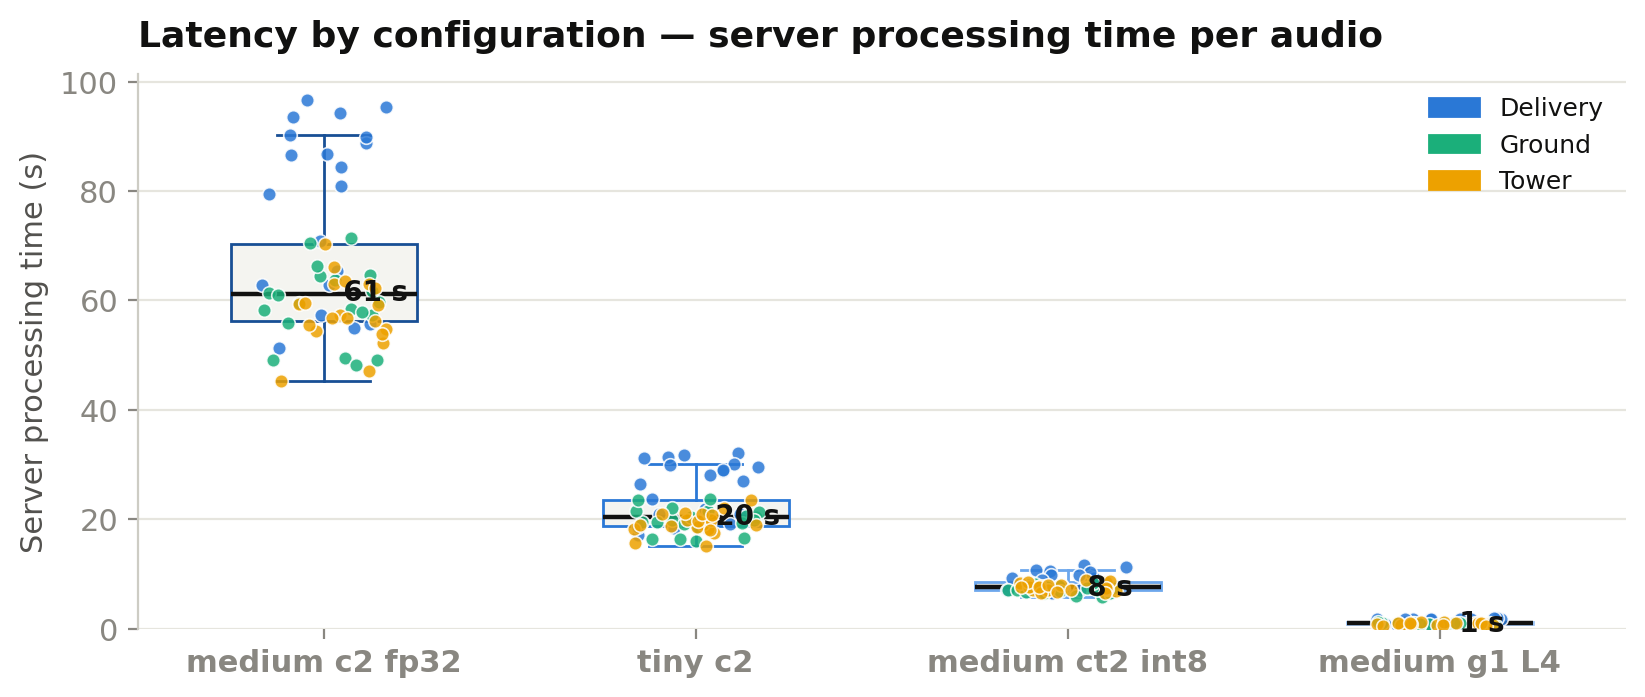
\includegraphics[width=\textwidth]{figures/chart_latency_by_config.png}
\caption{Per-audio processing time across three hardware configurations.
The GPU L4 tier (g1) achieves a median of 1.0~s, enabling live use.}
\label{fig:latency_configs}
\end{figure}

\begin{figure}[htbp]
\centering
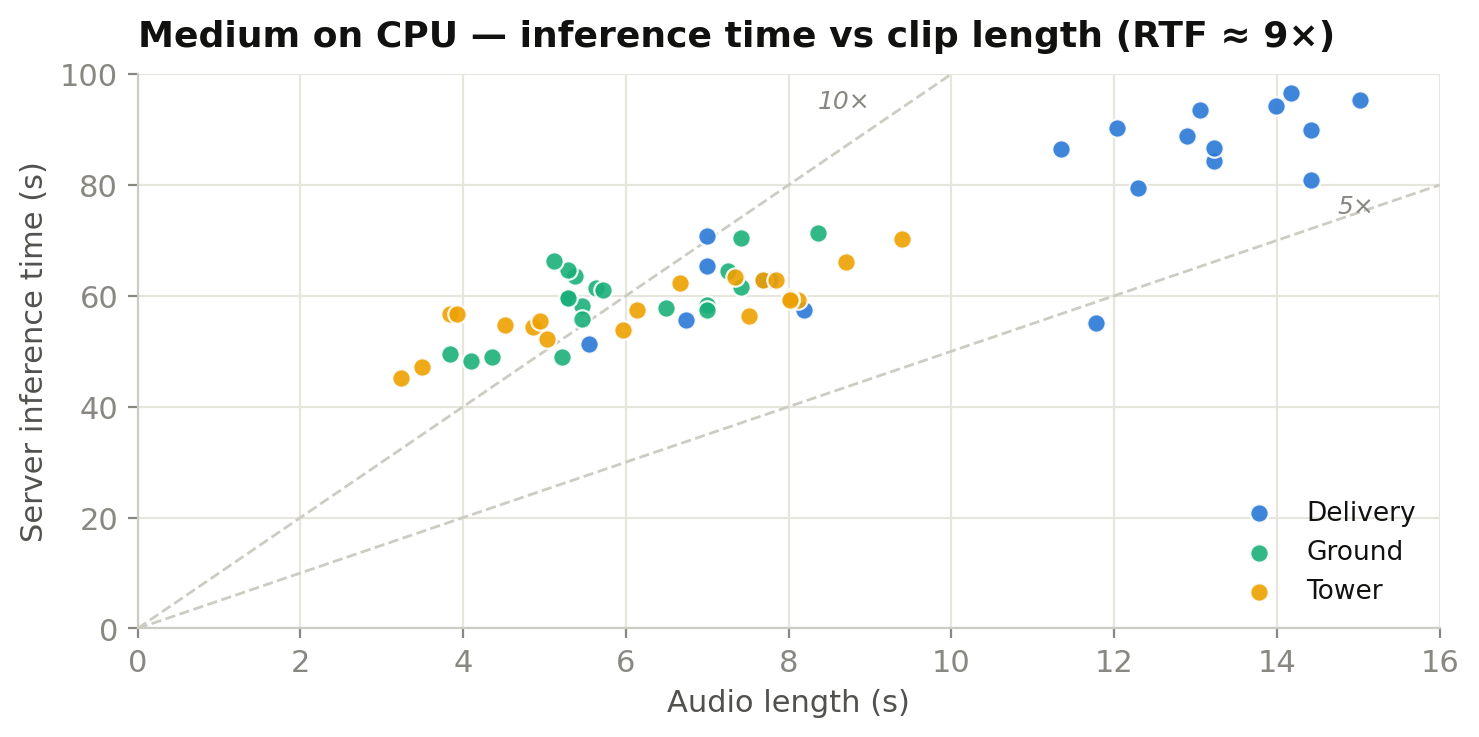
\includegraphics[width=0.7\textwidth]{figures/chart_rtf_scatter.png}
\caption{Real-Time Factor vs.\ utterance duration for the medium model on the
baseline c2 configuration. RTF remains linear with duration (no outliers).}
\label{fig:rtf}
\end{figure}

\subsubsection{Context-Aware ASR: Session Lexicon Prompting}
\label{sec:context}

A key limitation of generic ASR on ATC speech is that many errors are not random
distortions but systematic substitutions of callsigns and procedure names that
lie outside the model's training distribution. Because a controller session
involves a known, small set of active callsigns and expected SIDs, this
information can be supplied as a decoder \texttt{initial\_prompt} — a short prefix
that biases the next-token distribution toward the session
vocabulary~\cite{radford2023whisper}.

Three context modes were evaluated:

\begin{description}
  \item[\texttt{none}] No prompt at all. The model transcribes from a cold start.
  \item[\texttt{generic}] A fixed prompt of 11 realistic ATC exchanges
        (callsigns, QNH, squawk, runway, flight level), shared across all sessions.
  \item[\texttt{session}] The generic prompt extended with two sentences listing
        the active callsigns and expected SIDs for the current controller position
        (e.g., ``Active callsigns: RYR473, IBE5471, VLG32A. Expected SIDs:
        BELEN1G, NANDO3R, DVOR2G.'').
\end{description}

The effect is measured not through aggregate WER — which is diluted by common
words shared with the reference — but through entity-level accuracy: the fraction
of utterances in which the correct callsign and SID survive the full pipeline as
exact ICAO tokens. Table~\ref{tab:entity_accuracy} and
Figure~\ref{fig:entity_accuracy} present the results.

\begin{table}[htbp]
\caption{Entity-level accuracy with and without session context, for both the
CTranslate2 int8 (ct2) and GPU fp16 (g1) backends.}
\label{tab:entity_accuracy}
\centering
\begin{tabular}{llrrr}
\toprule
Backend & Context & Callsign acc. & SID acc. & LLM calls \\
\midrule
ct2 & none    & 65.0\% & 8.3\%  & 0  \\
ct2 & session & 81.7\% & 58.3\% & 7  \\
g1  & none    & 66.7\% & 8.3\%  & 0  \\
g1  & session & 86.7\% & 41.7\% & 10 \\
\bottomrule
\end{tabular}
\par\bigskip
\footnotesize Callsign accuracy: fraction of the 60 utterances where the correct ICAO callsign appears as an exact token in the final transcription. SID accuracy: fraction of the 12 utterances that contain a SID where the canonical SID name survives exactly. LLM calls: number of utterances where the deterministic pipeline fell below the rapidfuzz threshold of~80 and the Gemini fallback was invoked.
\end{table}

Session context lifts callsign accuracy by 15--20~percentage points across both
backends and multiplies SID accuracy by a factor of five to seven. Tower callsigns
reach 100\% under session context on the GPU tier. The residual gap between the
CTranslate2 and GPU backends on SID recovery (58.3\% vs.\ 41.7\%) is explained by
a known implementation issue: \texttt{initial\_prompt} token IDs remain on the CPU
when the model resides on \texttt{cuda:0}, triggering a silent fallback that
discards the prompt. The CTranslate2/faster-whisper backend, which natively
handles the prompt on the correct device, therefore benefits fully from the
session lexicon. A one-line fix is pending; re-measurement of the g1-session cell
is planned immediately after the patch.

The LLM fallback rescued 7 utterances on the ct2 backend and 10 on the g1 backend
— cases where the deterministic fuzzy match could not confidently resolve the
entity. These include challenging examples such as ``via NINIX1W departure''
where the callsign VLG123 was correctly recovered only through the Gemini call.
Table~\ref{tab:wer_context} reports the overall WER reduction attributable to the
full post-processing pipeline.

\begin{table}[htbp]
\caption{WER before and after the deterministic correction pipeline, by
configuration and context mode. WER$_{\text{post}}$ compares reference and
hypothesis after identical ICAO canonicalisation.}
\label{tab:wer_context}
\centering
\begin{tabular}{llrrr}
\toprule
Backend & Context & WER$_{\text{raw}}$ & WER$_{\text{post}}$ & $\Delta$ \\
\midrule
ct2 & none    & 14.9\% & 29.5\% & $-$14.6 \\
ct2 & session & 14.6\% & 19.8\% & $-$5.2  \\
g1  & none    & 14.2\% & 26.4\% & $-$12.2 \\
g1  & session & 14.2\% & 18.9\% & $-$4.7  \\
\bottomrule
\end{tabular}
\par\bigskip
\footnotesize WER$_{\text{post}}$ is computed against a canonically normalised
reference (ICAO compaction of callsigns and SIDs), which reduces the reference
word count and inflates the percentage. The meaningful comparison is
WER$_{\text{post}}$(session) vs.\ WER$_{\text{post}}$(none): session context
reduces corrected WER by 9.7~pp (ct2) and 7.5~pp (g1). The negative $\Delta$
values for \texttt{none} mode indicate that canonicalisation exposes errors that
raw WER masks — entities that were transcribed incorrectly but happened to contain
the same number of words as the reference.
\end{table}

\begin{figure}[htbp]
\centering
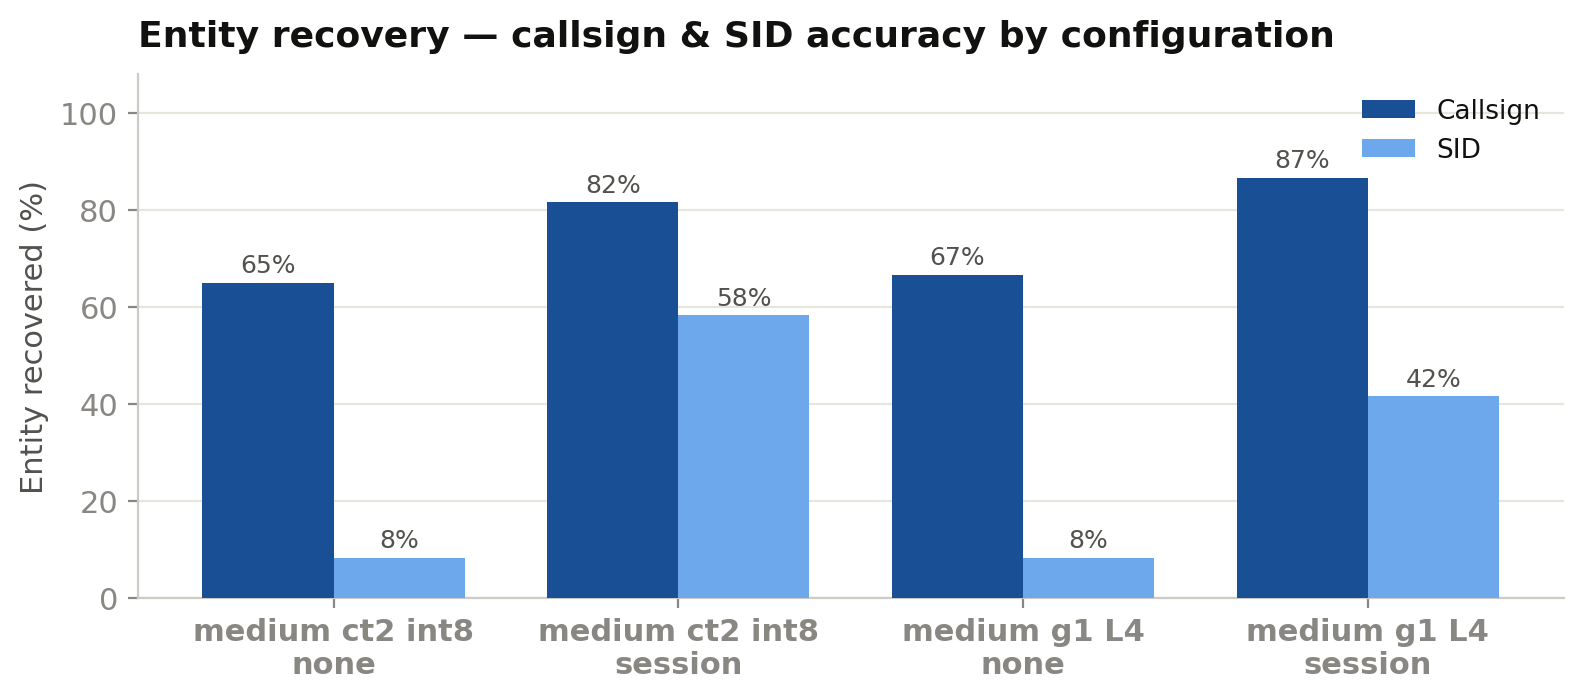
\includegraphics[width=\textwidth]{figures/chart_entity_accuracy.png}
\caption{Entity-level accuracy (callsign and SID) with and without session context.
Session-aware prompting raises callsign recovery from 65--67\% to 82--87\% and SID
recovery from 8\% to 42--58\%.}
\label{fig:entity_accuracy}
\end{figure}

\begin{figure}[htbp]
\centering

\includegraphics[width=\textwidth]{figures/chart_wer_context.png}
\caption{WER before and after post-processing, by configuration and context mode.}
\label{fig:wer_context}
\end{figure}

\subsubsection{Post-Processing Pipeline}

The raw Whisper output undergoes a deterministic five-stage correction pipeline
before being forwarded to the orchestrator (Figure~\ref{fig:pipeline}). Each stage
depends on the output of the previous one; the ordering is fixed:

\begin{enumerate}
  \item \textbf{Number normalisation.} Spoken digits are converted to figures
        only inside recognised ATC contexts: squawk codes
        (\emph{four five zero one} $\rightarrow$ \texttt{4501}), QNH
        (\emph{one zero one three} $\rightarrow$ \texttt{1013}), runway
        designators, altitude assignments, flight levels, and VHF frequencies.
        Digits appearing outside these patterns are left untouched.
  \item \textbf{Callsign correction.} A table of 13 regex patterns repairs known
        Whisper misrecognitions for common airline names (e.g.,
        \emph{bowling} $\rightarrow$ \emph{Vueling}). The airline-plus-phonetic-code
        span is then compacted to ICAO form (\emph{Ryanair four seven three}
        $\rightarrow$ \texttt{RYR473}) and fuzzy-matched against the active session
        callsigns using the rapidfuzz library with a score threshold of~80.
        Unrecognised airlines retain their spoken name.
  \item \textbf{SID normalisation.} Two patterns — the phrase form
        \emph{via BELEN one GOLF departure} and the bare token form
        \texttt{BELEN1G} — are matched and fuzzy-snapped to
        \texttt{session\_sids} using the same rapidfuzz threshold.
  \item \textbf{Phonetic letter compaction.} Isolated ICAO phonetic words
        (\emph{alpha}, \emph{bravo}) are reduced to single letters
        (\texttt{A}, \texttt{B}), primarily for taxiway and stand identifiers.
        This stage runs last so that spelled-out letters needed by the SID stage
        are not consumed prematurely.
  \item \textbf{LLM entity-mapping fallback.} When the deterministic fuzzy match
        falls below the 80-point threshold in session mode, a single targeted call
        to Gemini Flash (temperature~0.0, 8~s timeout) is made with a strict
        prompt: replace \emph{only} the mis-transcribed callsign or SID with the
        correct candidate from the session lists, leaving every other word
        unchanged. The fallback is fail-open: any error returns the deterministic
        result. In the benchmark, this step rescued 10 out of 60 difficult cases
        on the GPU tier and 7 on the CTranslate2 tier.
\end{enumerate}

\begin{figure}[htbp]
\centering
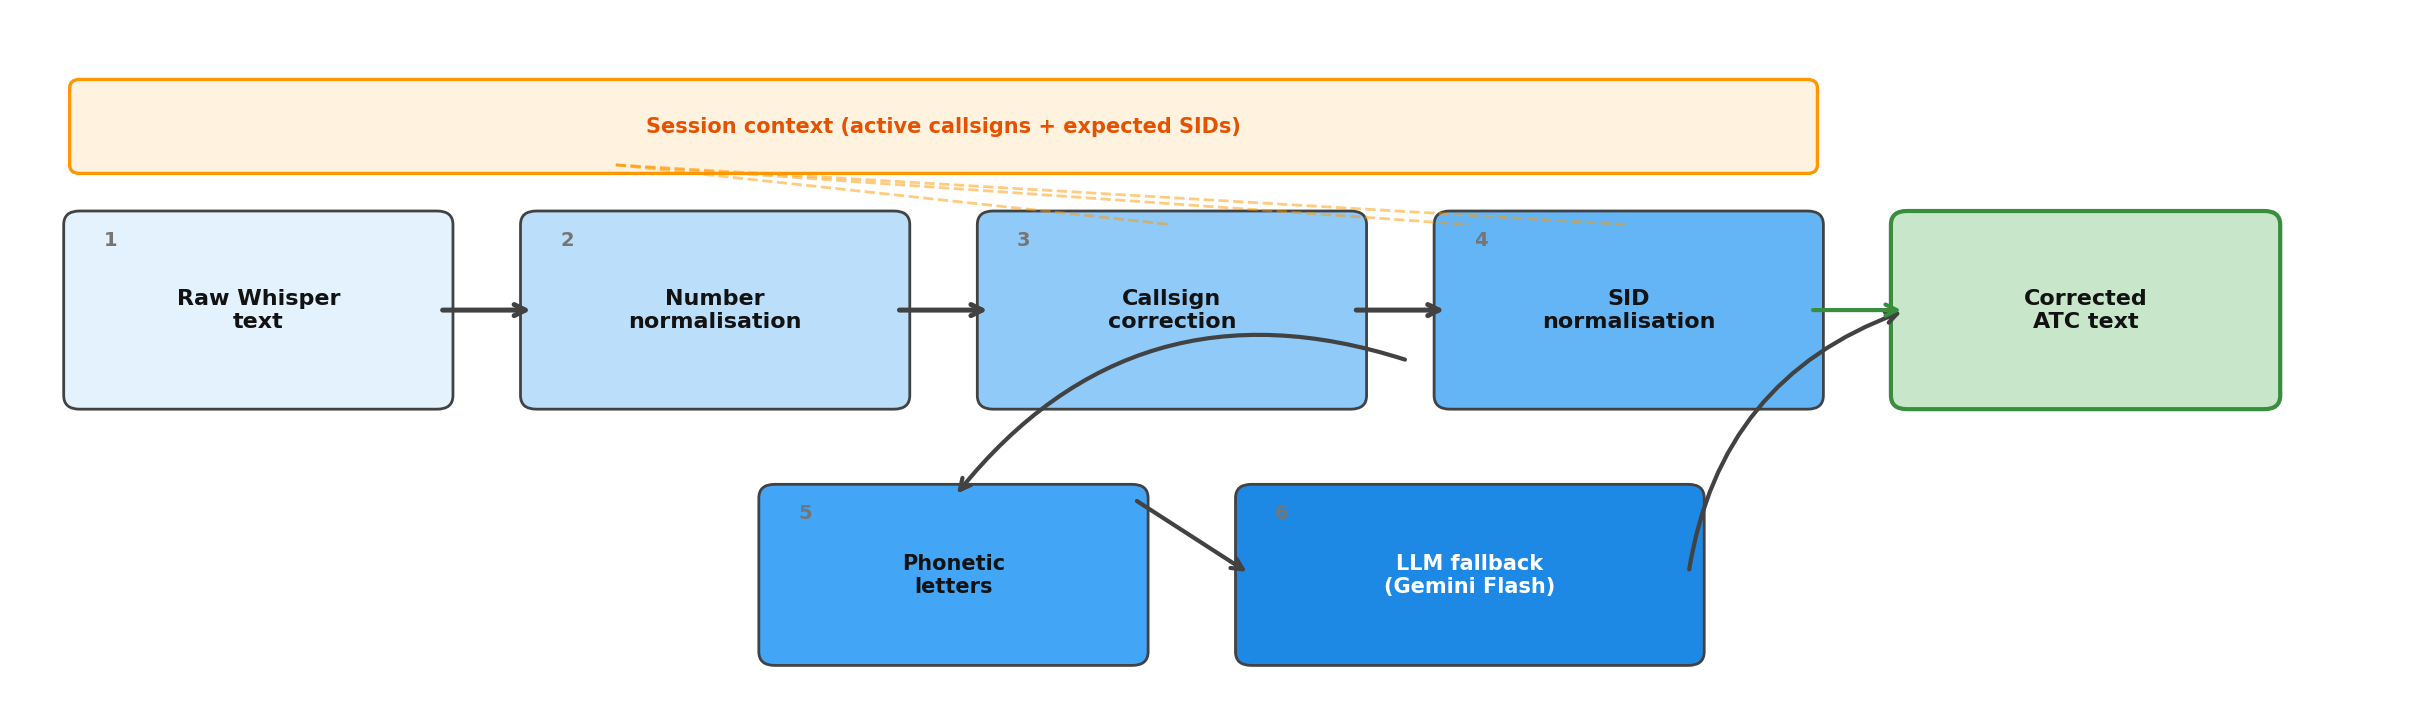
\includegraphics[width=0.75\textwidth]{figures/pipeline_asr.png}
\caption{Five-stage post-processing pipeline. Numbers, callsigns, SIDs, and
phonetics are normalised deterministically; a Gemini Flash call handles the
remaining unresolved entities only in session mode. The LLM is fail-open and
never invents values.}
\label{fig:pipeline}
\end{figure}

Critically, the fuzzy-snap stages never invent entity names: a fuzzy match is
accepted only when rapidfuzz reports a similarity $\ge 80$ against a
caller-supplied session entry. Without a session list, correction stops at the
compacted-but-unverified form. This design constraint ensures that the pipeline
is safe to run automatically in production — it degrades gracefully rather than
substituting plausible but incorrect values.

\subsubsection{Error Analysis and Quantisation Tradeoffs}

To characterise the ASR error profile, the per-utterance Word Error Rate was
decomposed into substitutions (S), deletions (D), and insertions (I) for each
controller position under the baseline medium/fp32/c2 configuration (see
Table~\ref{tab:summary_medium}).

Figure~\ref{fig:error_composition} presents the same data visually. Substitutions
overwhelmingly dominate the error budget. In Delivery, 48 of 68 errors are
substitutions — the model captures the acoustic signal but maps it to an
incorrect lexical entry (\emph{Departure} $\rightarrow$ \emph{Apache},
\emph{BELEN} $\rightarrow$ \emph{Ville}). Deletions are negligible (none in
Tower, 14 of 517 in Delivery), confirming that the audio signal is fully captured.
The error profile suggests that the dominant failure mode is recoverable through a
supplementary vocabulary — the direct motivation for the session-context mechanism
described in Section~\ref{sec:context}.

\begin{figure}[htbp]
\centering
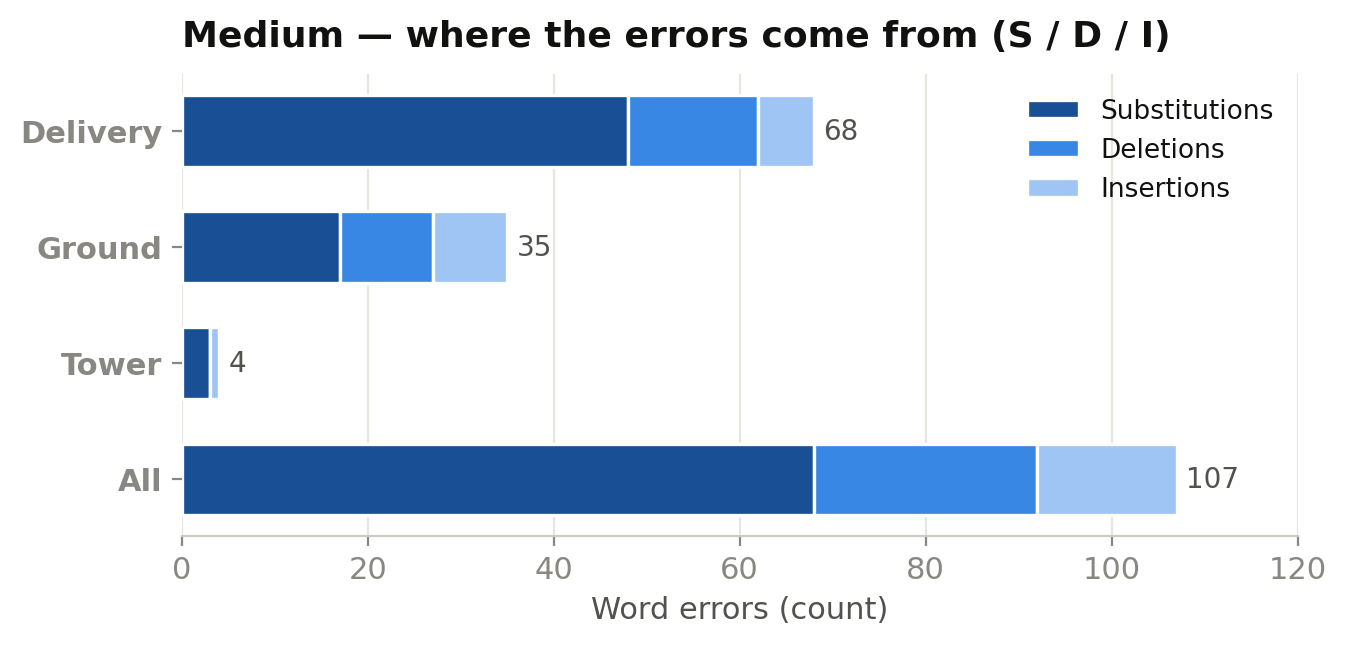
\includegraphics[width=\textwidth]{figures/chart_error_composition.png}
\caption{Error composition (substitutions, deletions, insertions) by controller
position for the medium model. Substitutions dominate, especially in Delivery
(48 of 68 total errors). Deletions are rare, indicating that the model
captures the audio signal without loss.}
\label{fig:error_composition}
\end{figure}

The per-utterance distribution (Figure~\ref{fig:wer_distribution}) reveals a
strongly bimodal pattern: 20 of 60 utterances are transcribed without a single
error, while a handful of long, lexically dense Delivery and Ground transmissions
drive the tail (worst case: \texttt{gnd\_020} at 50\% WER). This distribution
suggests that targeted vocabulary augmentation, not a fundamentally more powerful
acoustic model, is the most efficient path to closing the remaining gap.

\begin{figure}[htbp]
\centering
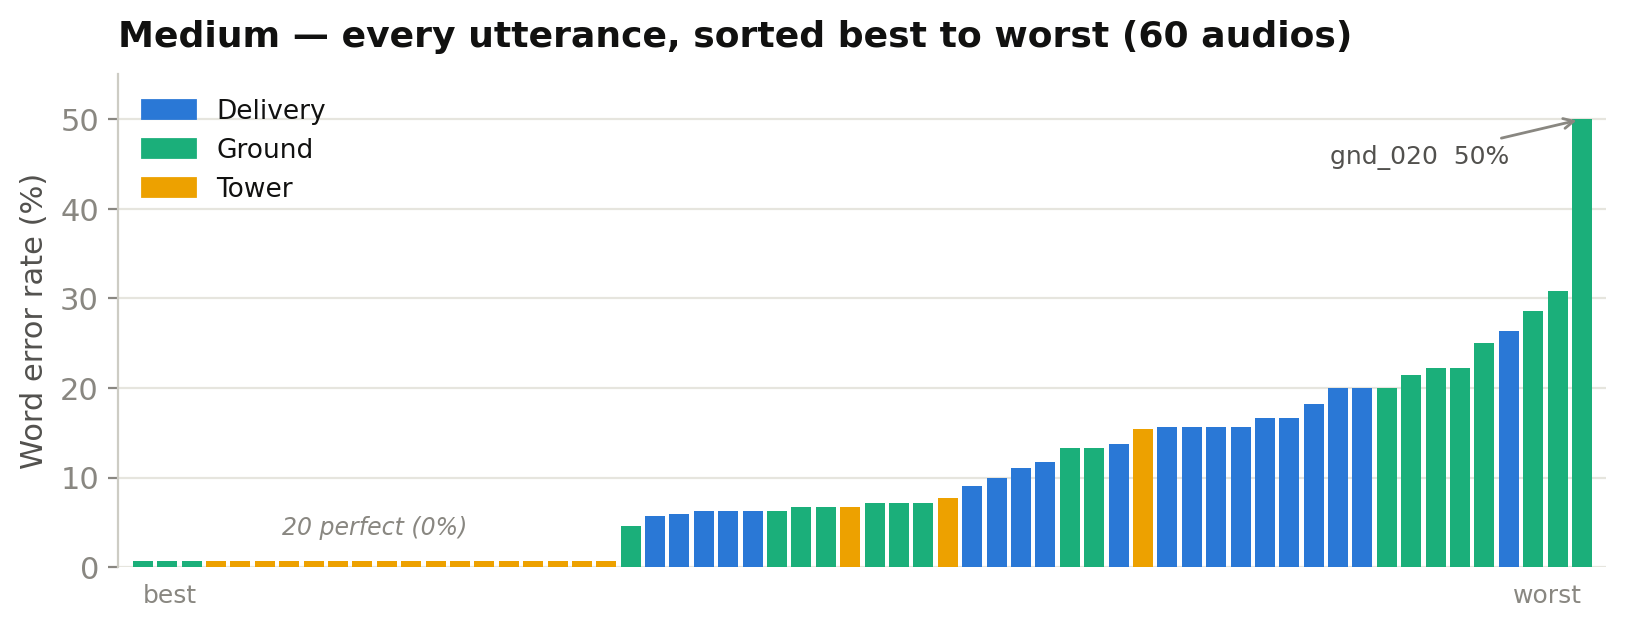
\includegraphics[width=\textwidth]{figures/chart_wer_distribution.png}
\caption{Per-utterance WER distribution for the 60 benchmark transmissions.
Twenty utterances achieve perfect 0\% WER; the tail is driven by a small number
of difficult Ground and Delivery samples.}
\label{fig:wer_distribution}
\end{figure}

A secondary finding concerns numerical precision. The same medium model was run
under three quantisation regimes (Table~\ref{tab:quantisation}): fp32 on CPU
(micro WER~9.8\%), int8 via CTranslate2 (14.0\%), and fp16 on GPU (13.5\%). The
4.2-percentage-point gap between fp32 and fp16 is measurable and consistent with
the known sensitivity of transformer decoders to half-precision
accumulation~\cite{nandakumar2024mixed}; the int8 figure lands between them
(Table~\ref{tab:quantisation}). While fp16 on GPU remains the only configuration
fast enough for live use, future work with the large-v3 model may widen the
accuracy margin enough to absorb the quantisation penalty without net loss
compared to the current medium/fp32 pipeline.

\begin{table}[htbp]
\caption{Micro WER under three quantisation regimes for the medium model. fp32 on
CPU achieves the highest accuracy; fp16 on GPU is 4.2~pp worse but 60$\times$
faster.}
\label{tab:quantisation}
\centering
\begin{tabular}{lrrrr}
\toprule
Precision & Backend & Hardware & Micro WER & Speedup vs.\ c2 \\
\midrule
fp32 & transformers (HF)  & 2~vCPU      & 9.8\%  & 1$\times$  \\
int8 & CTranslate2         & 8~vCPU      & 14.0\% & $\sim$7$\times$  \\
fp16 & transformers (HF)  & L4~GPU      & 13.5\% & $\sim$60$\times$ \\
\bottomrule
\end{tabular}
\end{table}

\endinput
  % 3.1 Automatic Speech Recognition

\subsection{ATC Agents: Delivery, Ground, and Tower}
\label{sec:agents}

[Placeholder — agent design, prompt structure, stateless design rationale,
Gemini Flash integration.]

\subsection{Orchestrator and Aircraft State Machine}
\label{sec:orchestrator}

[Placeholder — PostgreSQL state tracking, Redis real-time state,
DEL→GND→TWR lifecycle, ATC phase transitions.]

\subsection{X-Plane 12 Integration}
\label{sec:xplane}

[Placeholder — XPPython3 plugin, aircraft spawning, taxiway graph routing,
motion along taxi routes.]

\subsection{Evaluation Corpora}
\label{sec:corpora}

[Placeholder — pilot-readback-corpus (300 controller transmissions),
agent validation corpus (142 entries), audio recording setup.]

% =====================================================================
\section{Results}
\label{sec:results}

\subsection{ASR Benchmark}

The ASR results are presented in detail in Section~\ref{sec:context}
(Session~3.1.3) and summarised here. The key findings are:

\begin{itemize}
    \item The tiny Whisper model (38M) is unusable for ATC (620\% WER) due to
          looping hallucination; the medium model (770M) achieves 9.8\% WER
          (fp32), sufficient for downstream agent processing.
    \item GPU inference (NVIDIA L4, fp16) reduces latency to 1.0~s median
          (60$\times$ over CPU fp32), enabling live use.
    \item Session context improves callsign accuracy from 65--67\% to 82--87\%
          and SID accuracy from 8\% to 42--58\%, through a combination of
          decoder prompting and a deterministic-plus-LLM post-processing
          pipeline.
    \item The LLM fallback rescued 7--10 of 60 difficult cases where the
          deterministic fuzzy match could not confidently resolve an entity.
\end{itemize}

\subsection{Agent Readback Quality}

[Placeholder — agent evaluation: latency percentiles, schema validity,
field-by-field validation of squawk, altitude, runway, SID.]

% =====================================================================
\section{Discussion}
\label{sec:discussion}

[Placeholder — interpretation of results, comparison with prior work,
practical implications, limitations, known bugs (initial\_prompt GPU issue).]

% =====================================================================
\section{Conclusions}
\label{sec:conclusions}

[Placeholder — summary of contributions, future work (large-v3 benchmark,
full 300-audio corpus, Wilcoxon test).]

% =====================================================================
% Bibliography
% =====================================================================
\bibliographystyle{mdpi}
\bibliography{references}

\end{document}
